\documentclass[12pt,a4paper]{article}
\usepackage[top=1in, bottom=1in, left=1in, right=1in]{geometry}
\geometry{headheight=15pt}
\usepackage{fancyhdr}\pagestyle{fancy}\rhead{(your UID) (your name)}\lhead{Math 151B - homework 2}
\usepackage{amsmath,amssymb,amsthm,amsfonts,microtype,stmaryrd}
\usepackage{hyperref}\hypersetup{linktocpage,colorlinks}\hypersetup{urlcolor=blue}
\usepackage{graphicx} \graphicspath{}
% --Example:
% 	\includegraphics[scale=0.5]{picture name}

%%%%%%%%%%%%%%%%%%%%%%%%%%%%%%%%%%%%%%%%%%%%%%%%%%%%%%%%%%%%%%%%%%%%%%%%%%%%%%%%%%%%%%%%%%%%%%%%%%%%%%%%%%%%%%%%%%%%%%%%%%%%%%%%%%%%%%%%%%%%%%%%%%%%%%%%%%%%%%%%%%%%%%%%%%%%%%%%%%%%%%%%%%%%%%
\begin{document}
\title{Your Title}
\date{\today}
\author{Your Name}
\maketitle

\subsubsection*{[Textbook Problem \#4.2.1]}
\noindent (The \texttt{\textbackslash noindent} command disables the automatic indentation at the beginning of each paragraph. )

(Here's an example of automatic indentation.) \\
\\
(\texttt{\textbackslash\textbackslash} breaks 
a 
line; \\ enter 
does 
nothing.)
$$ \mbox{(math formula)}\footnote{Aliases for most mathematical symbols can be found at \url{https://www.artofproblemsolving.com/wiki/index.php/LaTeX:Symbols}} \int_a^b f'(x)dx = f(b) - f(a) $$
$$ \mbox{(matrix and vector) } \mathbf{A} = \left[
\begin{array}{cccc}
a_{11} & a_{12} & \cdots & a_{1n}\\
a_{21} & a_{22} &  & \\
\vdots & & \ddots &\\
a_{n1} & & & a_{nn}\end{array}
\right], 
\mathbf{v} = \left[
\begin{array}{c}
v_1\\
v_2\\
\vdots\\
v_n\end{array}
\right]$$
\begin{align*}
\mbox{(aligned equations) } \sin(2\theta) &= \sin(\theta + \theta) \\
&= \sin\theta\cos\theta + \cos\theta\sin\theta \\
&= 2\sin\theta\cos\theta
\end{align*}



\newpage\subsubsection*{[Programming Problem 1]}
\begin{verbatim}
%% The package verbatim helps you format programming codes in your LaTeX file......
%% Note that it doesn't automatically break lines.
x = A\b;
fprintf('Hello world');
\end{verbatim}


\begin{center}
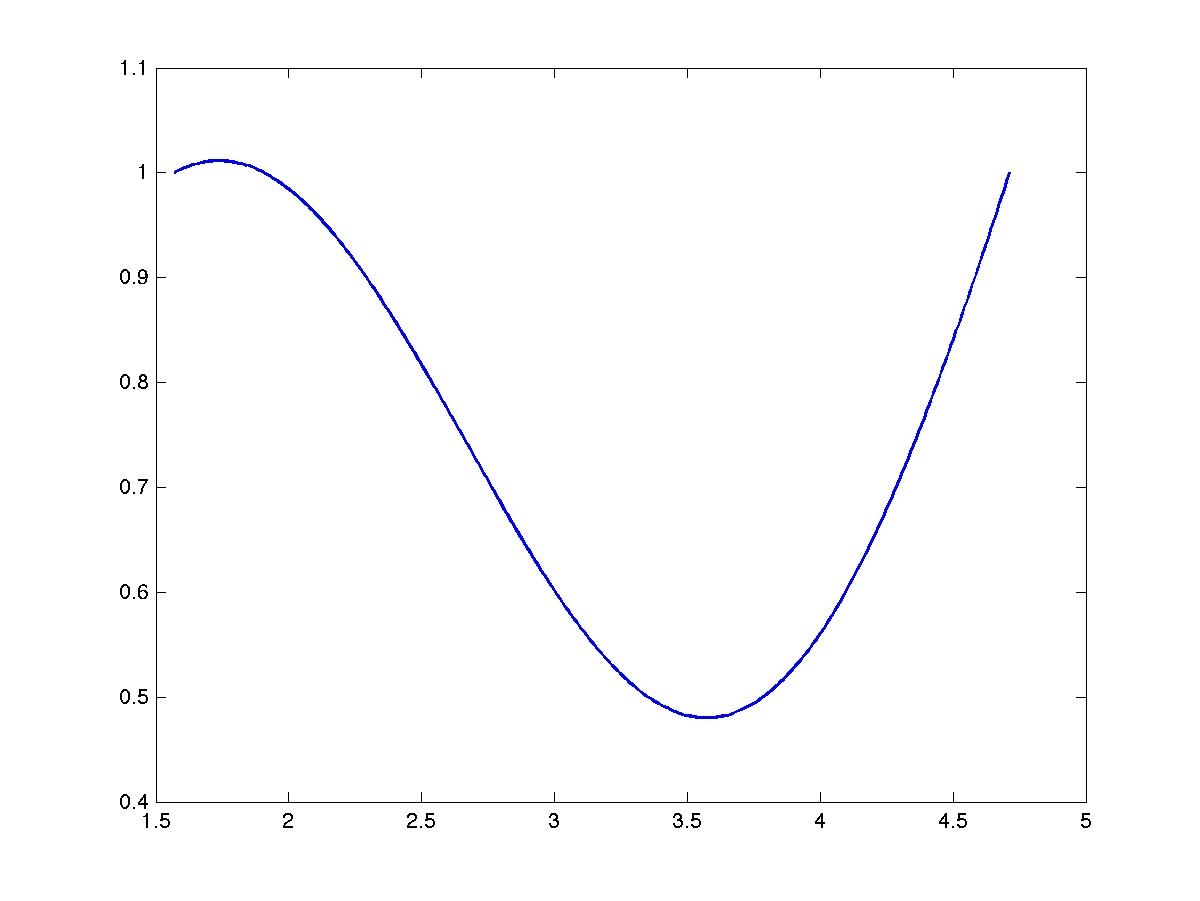
\includegraphics[scale=0.33]{sample_fig.jpg}\\
The center environment helps you locate your figures and captions in the middle. 
\end{center}
\end{document}
